\documentclass[12pt]{article}
\usepackage[T1]{fontenc}
\usepackage[utf8]{inputenc}
\usepackage[ngerman]{babel}
\usepackage{lmodern}
\usepackage{latexsym}
\usepackage{amsfonts}
\usepackage{amssymb}
\usepackage{amsmath}

%Richtiger Differentialquotient
\newcommand*\dx{\: \mathrm{d}x}
\newcommand*\dy{\: \mathrm{d}y}
\newcommand*\dt{\: \mathrm{d}t}
\newcommand*\du{\: \mathrm{d}u}
\newcommand*\da{\: \mathrm{d}a}
\newcommand*\dz{\: \mathrm{d}z}
\newcommand*\dr{\: \mathrm{d}r}
\newcommand*\dth{\: \mathrm{d}\Theta}

% Bilddateien einlesen
\usepackage{graphicx}

%Satzspiegel
\usepackage[automark]{scrlayer-scrpage}
\pagestyle{scrheadings}
\clearscrheadfoot
\ihead{Florian Wolf, Julian Weigert; Blatt 9} %linke Kopfzeile %Klasse hinzufügen!
\ohead{Nicolai Locher} %rechte Kopfzeile
\cfoot{\pagemark}

\topmargin -2cm
\textheight 25cm
\textwidth 16.0 cm
\oddsidemargin -0.1cm



\begin{document}
\subsection*{Aufgabe 26:}
Im folgenden Schaubild werden von der Funktion 
\begin{align*}
p: \mathbb{C} \to \mathbb{C},\; p(z) = 1 + z + \frac{z^2}{2} + \frac{z^3}{6} + \frac{z^4}{24} + \frac{z^5}{120}
\end{align*}
die Bereiche
\begin{align*}
B_n = \{ z \in \mathbb{C}: n-1 \leq |p(z)| < n \}, \; n = 1, \ldots, 10
\end{align*}
gezeichnet.
\begin{figure}[h!]
\centering
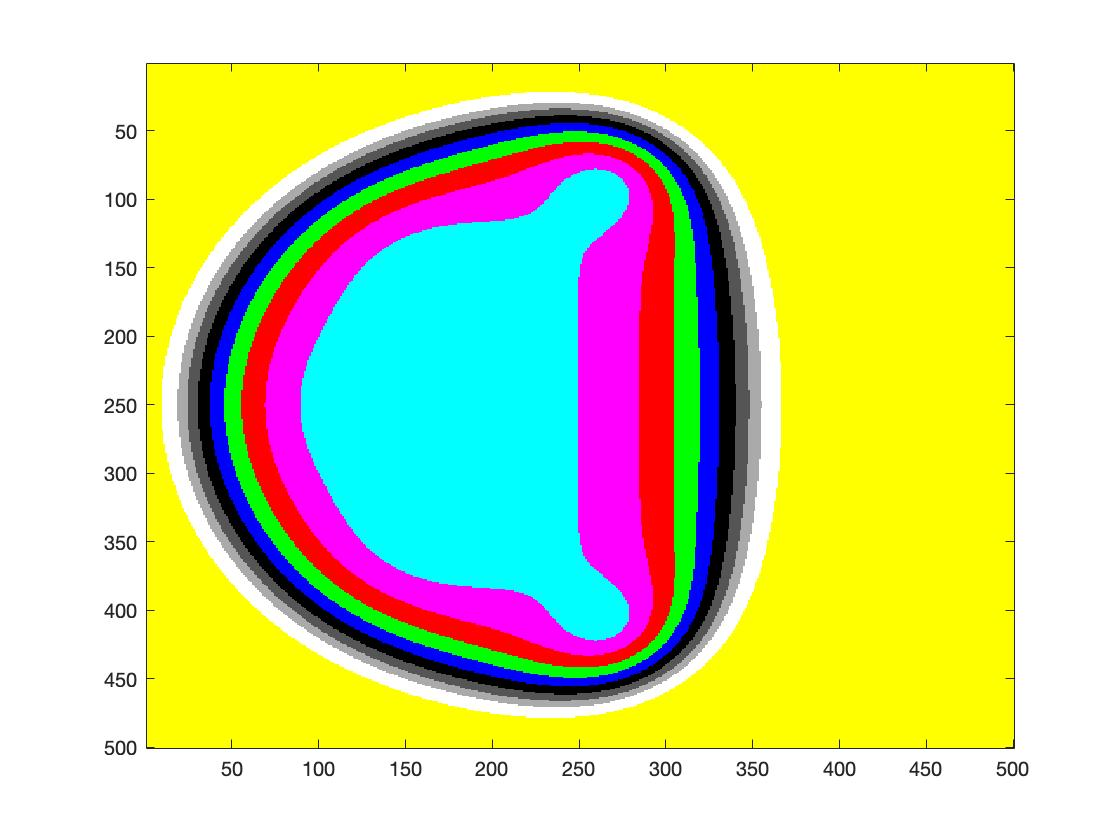
\includegraphics[scale=0.4]{pictureExercive9_1}
\caption{Bildbereiche der oben definierten Funktion.}
\end{figure}
\end{document}